\subsection{Improved K-Means}
\label{subsec:improvedkmeansresults}

This section provides an overview of the results obtained from the improved K-Means algorithms implemented, Global K-Means and G-Means.

\subsubsection{Global K-Means}
\label{subsec:globalkmeansresults}

\begin{figure}[h!]
    \centering
    \includegraphics[width=0.5\textwidth]{figures/interactions_global_kmeans.png}
    \caption{Hyperparameter interactions for Global K-Means}
    \label{fig:interactions-global-kmeans}
\end{figure}

We found that the number of clusters had the most significant impact on the F-measure, as shown in Figure \ref{fig:interactions-global-kmeans}. For both the Mushroom and Hepatitis datasets, the F1 score was
highest when number of clusters set to 2, and steadily decreased as the number of clusters increased. For the Vowel dataset, the F1 score was lowest
with a small number of clusters, and increased as the number of clusters increased, peaking at number of clusters set to 11.
These results are consistent with the number of classes in each dataset— 2 for Mushroom and Hepatitis, and 11 for Vowel.

The tolerance and $max_iteration$ parameters both had a negligable impact on the F1 score.
One possible explanation for this is that, in Global K-Means, the tolerance parameter primarily
influences the convergence criteria of the K-Means subroutine used at each step of the algorithm.
As long as K-Means converges successfully for a given number of clusters, the overall clustering
results remain largely unaffected. Similarly, the $max_iterations$ parameter acts as a safeguard to prevent
excessively long runtimes but does not directly influence the final cluster placements, provided that
convergence is reached within the allowed iterations. These findings suggest that factors such as
the initial placement of centroids and the maximum number of clusters are more critical to the
performance of Global K-Means than the tolerance or max iterations parameters.

\subsubsection{G-Means}
\label{subsec:gmeansresults}

\begin{figure}[h!]
    \centering
    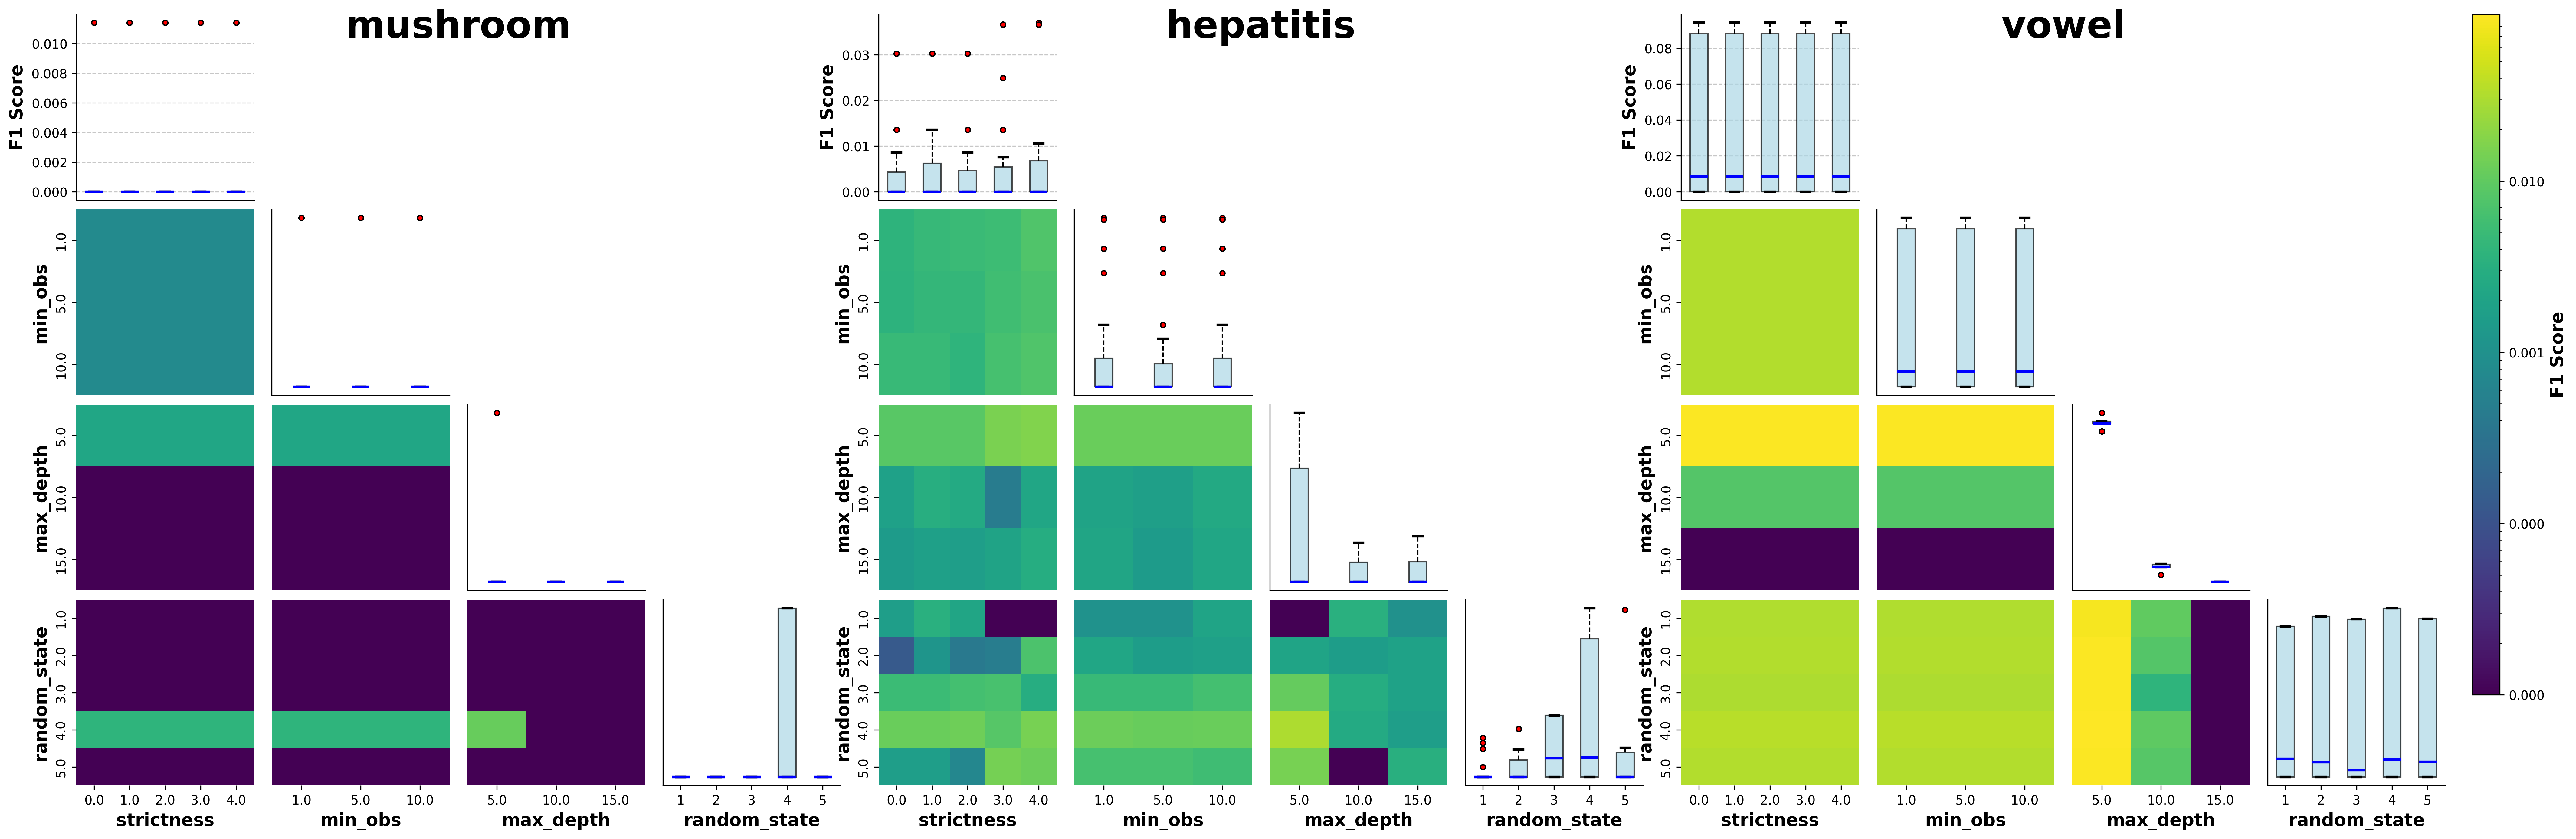
\includegraphics[width=0.5\textwidth]{figures/interactions_gmeans.png}
    \caption{Hyperparameter interactions for G-Means}
    \label{fig:interactions_gmeans}
\end{figure}

Compared to Global K-Means, the results are more varied for G-Means as shown in Figure \ref{fig:interactions_gmeans}.

The F1 score for the Mushroom dataset remains consistently low across all configurations of the hyperparameters.
While there are some outliers, the overall clustering performance is poor, with F1 scores close to zero for most parameter combinations.
The heatmaps show little variation across hyperparameter values, suggesting that changes to $max_depth$, strictness, or $min_obs$ have
negligible impact on the clustering outcome. The bar plot for $random_state$ indicates some sensitivity to initialization, but even
the best cases fail to produce meaningful clusters. These results suggest that G-Means is ill-suited for the Mushroom dataset.

For the Hepatitis dataset, the F1 score shows greater variability across hyperparameter configurations. The heatmaps reveal that
$max_depth$ and $random_state$ have more noticeable impacts on clustering performance, with specific combinations producing
better results. The box plots indicate significant outliers, particularly for strictness and $max_depth$, suggesting these parameters
introduce instability. Overall, these results show G-Means hyperparameter combinations are sensitive for this dataset,
highlighting the need for careful selection to optimize performance. Despite this, the F1 scores remain low, indicating G-Means
cannot accurately predict the clusters in the Hepatitis dataset.

The F1 score remains consistently low across all hyperparameter configurations for the Vowel dataset.
The heatmaps suggest that $max_depth$ is the most significant hyperparameter, with lower levels producing the best results.
Having said this, the results are still poor. The box plots show negligible variability for most parameters, with no significant outliers.
These results indicate that G-Means struggles to produce meaningful clusters for this dataset,
likely due to the dataset's complexity and the algorithm's limitations in handling high-class scenarios.